\documentclass[catalan, a4paper, 12pt, titlepage]{article}
\usepackage{babel}
\usepackage{graphicx}
\usepackage{fontawesome5}
\graphicspath{ {./img/} }
\usepackage{mathptmx}
\renewcommand{\baselinestretch}{1.5}
%\usepackage{isolatin1}

%tikz
\usepackage{tikz}
\usetikzlibrary{mindmap}

%hyperref
\usepackage[pdftex,pdfpagelabels,bookmarks,hyperindex,hyperfigures,hidelinks]{hyperref}

\usepackage{termcal}

% Few useful commands (our classes always meet either on Monday and Wednesday
% or on Tuesday and Thursday)

\newcommand{\MWClass}{%
\calday[Monday]{\classday} % Monday
\skipday % Tuesday (no class)
\calday[Wednesday]{\classday} % Wednesday
\skipday % Thursday (no class)
\skipday % Friday
\skipday\skipday % weekend (no class)
}

\newcommand{\TRClass}{%
\skipday % Monday (no class)
\calday[Tuesday]{\classday} % Tuesday
\skipday % Wednesday (no class)
\calday[Thursday]{\classday} % Thursday
\skipday % Friday
\skipday\skipday % weekend (no class)
}

\newcommand{\MTRFClass}{%
	\calday[Monday]{\classday}
	\calday[Tuesday]{\classday}
	\skipday % Dimecres
	\calday[Thursday]{\classday}
	\calday[Friday]{\classday}
\skipday\skipday % weekend (no class)
}

\newcommand{\Holiday}[2]{%
\options{#1}{\noclassday}
\caltext{#1}{#2}
}

\usepackage{lastpage}

\usepackage{fancyhdr}

\fancyhead[L]{\small{Programació didàctica - Gestió de bases de dades}}
\fancyhead[R]{\small{Jaume Barceló Vicens}}
\fancyfoot[C]{\small{Pàgina \thepage\ de \pageref{LastPage}}}

% Uncomment to remove the header rule
\renewcommand{\headrulewidth}{0pt}

\title{Una programació didàctica de \\
gestió de bases de dades\\
	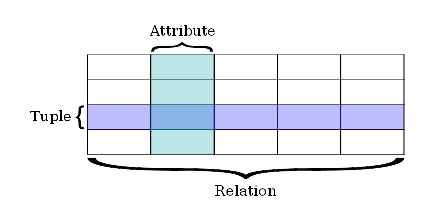
\includegraphics[width=10cm]{database.eps}
	}

\author{
	Jaume Barceló Vicens
	DNI 43135949R\\
	Professors d'ensenyament secundari (0590)
	Especialitat informàtica}

\date{
	Família professional informàtica \\
	Cicle formatiu de grau superior d’Administració de Sistemes Informàtics en Xarxa\\
	Mòdul professional de gestió de bases de dades\\
	Codi 0372 170h (+90h d'anglès)\\
	http://github.com/jbarcelo/programacio\_didactica\_gbd \\
	Llicència CC-BY-SA 4.0 \faCreativeCommons\ \faCreativeCommonsBy\ \faCreativeCommonsSa}

\setcounter{tocdepth}{3}

\begin{document}

\pagestyle{empty}

\maketitle

\tableofcontents 

\pagestyle{fancy}

\section{Introducció}

Aquesta és la programació didàctica del mòdul ``Gestió de bases de dades'' (codi 0372) del cicle formatiu de ``Tècnic superior en administració de sistemes i xarxes'' que s'imparteix al CIFP Francesc de Borja Moll el curs escolar 2021-2022.

Aquesta programació tracta de reflectir l'experiència de la impartició d'aquest mateix mòdul durant el curs 2019-2020. A més, aquesta programació didàctica es presenta com una guia oberta i flexible, sobre la que es poden fer tants canvis com siguin necessaris per adaptar-se a la realitat del grup d'alumnes i del curs en general.

\section{Normativa.}

Aquesta programació s'ha desenvolupat tenint en compte la següent normativa estatal:
\begin{itemize}
	\item Llei Orgànica 2/2006, de 3 de maig, d'Educació, que assenyala que el Gobierno de España, prèvia consulta a les comunitats autònomes, establirà les titulacions de formació professional i els aspectes bàsics del currículum.
	\item Llei Orgànica, 8/2013, de 9 de desembre per a la millora de la qualitat educativa i que modifica la LOE. Val a dir que ens trobem en una etapa de transició cap a la nova Llei Orgànica de Modificació de la LOE.
	\item Llei Orgànica 5/2002, de 19 de juny, de les Qualificacions i de la Formació Professional, que posa en marxa el Sistema Nacional de Qualificacions i Formació professional, desenvolupada pel Reial Decret 1128/2003, de 5 de setembre, modificat pel Reial Decret 1416/2005, de 25 de novembre, sobre el Catàleg Nacional de Qualificacions Professionals.
	\item Reial Decret 1147/2011, de 29 de juliol, pel qual s'estableix l'ordenació general de la formació professional basada en el Catàleg Nacional de Qualificacions Professionals.
	\item Reial Decret 1629/2009, de 30 d'octubre, pel qual s'estableix el títol de ``Tècnic Superior en Administració de Sistemes Informàtics en Xarxa'' i es fixen els seus ensenyaments mínims.
	\item Ordre EDU / 392/2010, de 20 de gener, per la qual s'estableix el currículum del cicle formatiu de grau superior corresponent al títol de ``Tècnic Superior en Administració de Sistemes Informàtics en Xarxa''.
\end{itemize}

En l'àmbit autonòmic considerem la següent normativa:
\begin{itemize}
	\item Decret 91/2012, de 23 de novembre, pel qual s'estableix l'ordenació general de la formació professional del sistema educatiu en el sistema integrat de formació professional a les Illes Balears.
	\item Ordre de la consellera d'Educació i Cultura de 13 de juliol de 2009 per la qual es regula l'organització i el funcionament dels cicles formatius de formació professional del sistema educatiu que s'imparteixen d'acord amb la Llei orgànica 2/2006, de 3 de maig, d'educació, a les Illes Balears, en la modalitat d'ensenyament presencial.
	\item Resolució del conseller d'Educació i Universitat de 18 d'abril de 2018 per la qual s'estableix el calendari escolar del curs 2018-2019 per als centres docents no universitaris de la comunitat autònoma de les Illes Balears.
\end{itemize}

Finalment, en l'àmbit del centre, considerem la següent normativa:
\begin{itemize}
	\item Projecte educatiu de centre (PEC) que planteja les intencions educatives i organitzatives del CIFP: las seva missió, visió i valors. I que inclou com a annexos el projecte lingüístic, el reglament d'organització i funcionament i la concreció curricular del centre.
\end{itemize}

\section{Contextualització}

Aquesta programació didàctica és per al mòdul Gestió de Bases de Dades del Cicle Formatiu de Grau Superior d'Administració de Sistemes Informàtics i Xarxes del Centre Integrat de Formació Professional Francesc de Borja Moll. 

A la comunitat Autònoma de les Illes Balears, la tipologia dels centres integrats ha estat reconeguda a partir de la Resolución del conseller d'educació i universitat de 24 de maig de 2018 per la qual es determina la tipologia dels centres docents públics no universitaris.

El centre es crea el curs 2019-20 amb estudis de doble torn i comparteix espais amb l'IES Nou Llevant. A més d'informàtica, hi trobam estudis de comerç i màrqueting, imatge personal, sanitat, i seguretat i medi ambient.

El CIFP Francesc de Borja Moll ofereix el grau mitjà i els tres graus superiors de la família professional d'informàtica. 
A més, ofereix programes d'FP dual tant per a ASIX com per a DAW.
La gran oferta formativa d'informàtica fa que aquest departament sigui molt nombrós, amb tots els avantatges i inconvenients que comporta.
Per una banda, hi ha una gran quantitat de coneixement i expertesa acumulats que permet aprendre i fer projectes que serien més difícils en un departament més petit.
Per una altra banda, a vegades pot ser difícil coordinar i posar d'acord tanta gent.

Un dels avantatges que suposa estar en un centre gran és que és possible per al professor impartir el mateix mòdul a diferents grups i, per tant, concentrar esforços.
Per exemple, el mateix professor pot tenir els grups d'ASIX i ASIX dual.
De totes maneres, el grup d'ASIX dual presenta certes particularitats ja que s'ha d'incorporar a la feina a mig curs i, en conseqüencia, reduir el temps que passa a l'institut.
L'alumnat haurà d'aprendre al lloc de feina part dels continguts i les competències del mòdul.
A més, durant els primers mesos de classe s'ha de proporcionar a l'alumnat de dual la formació necessària perquè pugui afrontar amb èxit les entrevistes i la incorporació al lloc de feina.
Al mateix temps, s'ha de tenir prou flexibilitat per redirigir el curs en cas que la incorporació a l'empresa no sigui possible per qualque esdeveniment inesperat, com per exemple una pandèmia.

\section{Objectius. Competències. Continguts.}

\subsection{Objectius generals}

Els objectius generals estableixen les capacitats que s'espera que els alumnes hagin assolit a final de curs. Segons el títol de tècnic superior en administració de sistemes informàtics en xarxa, s'estableixen els següents objectius. S'han marcat amb un símbol (\faCheck) aquells que es corresponen al mòdul de gestió de base de dades.

1. Analitzar l'estructura del programari de base, comparant les característiques i prestacions de sistemes lliures i propietaris, per administrar sistemes operatius de servidor.

2. Instal·lar i configurar el programari de base, seguint documentació tècnica i especificacions donades, per administrar sistemes operatius de servidor.

3. Instal·lar i configurar programari de missatgeria i transferència de fitxers, entre d'altres, relacionant-los amb la seva aplicació i seguint documentació i especificacions donades, per administrar serveis de xarxa.

\faCheck 4. Instal·lar i configurar programari de gestió, seguint especificacions i analitzant entorns d'aplicació, per administrar aplicacions.

\faCheck 5. Instal·lar i administrar programari de gestió, relacionant-lo amb la seva explotació, per implantar i gestionar bases de dades.

6. Configura dispositius maquinari, analitzant les seves característiques funcionals, per optimitzar el rendiment de el sistema.

7. Configura maquinari de xarxa, analitzant les seves característiques funcionals i relacionant-lo amb el seu camp d'aplicació, per a integrar equips de comunicacions.

8. Analitzar tecnologies d'interconnexió, descrivint les seves característiques i possibilitats d'aplicació, per configurar l'estructura de la xarxa telemàtica i avaluar el seu rendiment.

9. Elaborar esquemes de xarxes telemàtiques utilitzant programari específic per a configurar l'estructura de la xarxa telemàtica.

10. Seleccionar sistemes de protecció i recuperació, analitzant les seves característiques funcionals, per posar en marxa solucions d'alta disponibilitat.

11. Identificar condicions d'equips i instal·lacions, interpretant plans de seguretat i especificacions de fabricant, per supervisar la seguretat física.

12. Aplicar tècniques de protecció contra amenaces externes, tipificant i avaluant per assegurar el sistema.

\faCheck 13. Aplicar tècniques de protecció contra pèrdues d'informació, analitzant plans de seguretat i necessitats d'ús per assegurar les dades.

14. Assignar els accessos i recursos de sistema, aplicant les especificacions de l'explotació, per administrar usuaris

15. Aplicar tècniques de monitoratge interpretant els resultats i relacionant-los amb les mesures correctores per diagnosticar i corregir les disfuncions.

16. Establir la planificació de tasques, analitzant activitats i càrregues de treball de sistema per gestionar el manteniment.

17. Identificar els canvis tecnològics, organitzatius, econòmics i laborals en la seva activitat, analitzant les seves implicacions en l'àmbit de treball, per resoldre problemes i mantenir una cultura d'actualització i innovació.

18. Identificar formes d'intervenció en situacions col·lectives, analitzant el procés de presa de decisions i efectuant consultes per liderar les mateixes.

19. Identificar i valorar les oportunitats d'aprenentatge i la seva relació amb el món laboral, analitzant les ofertes i demandes de mercat per gestionar la seva carrera professional.

20. Reconèixer les oportunitats de negoci, identificant i analitzant demandes de mercat per crear i gestionar una petita empresa.

21. Reconèixer els seus drets i deures com a agent actiu en la societat, analitzant el marc legal que regula les condicions socials i laborals per participar com a ciutadà democràtic.

Els objectius generals als que contribueix el mòdul de gestió de bases de dades són: 4, 5 i 13.

\subsection{Competències professionals, personals i socials}

Les competències professionals, personals i socials d'aquest títol són les que es relacionen a continuació. 
S'han marcat amb un símbol les que es corresponen al mòdul de gestió de base de dades.

1. Administrar sistemes operatius de servidor, instal·lant i configurant el programari, en condicions de qualitat per assegurar el funcionament de el sistema.

2. Administrar serveis de xarxa (web, missatgeria electrònica i transferència d'arxius, entre d'altres) instal·lant i configurant el programari, en condicions de qualitat.

\faCheck 3. Administrar aplicacions instal·lant i configurant el programari, en condicions de qualitat per respondre a les necessitats de l'organització.

\faCheck 4. Implantar i gestionar bases de dades instal·lant i administrant el programari de gestió en condicions de qualitat, segons les característiques de l'explotació.

5. Optimitzar el rendiment de sistema configurant els dispositius maquinari d'acord amb els requisits de funcionament.

6. Avaluar el rendiment dels dispositius maquinari identificant possibilitats de millores segons les necessitats de funcionament.

7. Determinar la infraestructura de xarxes telemàtiques elaborant esquemes i seleccionant equips i elements.

8. Integrar equips de comunicacions en infraestructures de xarxes telemàtiques, determinant la configuració per assegurar la seva connectivitat.

9. Implementar solucions d'alta disponibilitat, analitzant les diferents opcions de mercat, per protegir i recuperar el sistema davant de situacions imprevistes.

10. Supervisar la seguretat física segons especificacions de fabricant i el pla de seguretat per evitar interrupcions en la prestació de serveis de sistema.

11. Assegurar el sistema i les dades segons les necessitats d'ús i les condicions de seguretat establertes per prevenir fallades i atacs externs.

12. Administrar usuaris d'acord a les especificacions d'explotació per garantir els accessos i la disponibilitat dels recursos de sistema.

\faCheck 13. Diagnosticar les disfuncions de sistema i adoptar les mesures correctives per restablir la seva funcionalitat.

14. Gestionar i / o realitzar el manteniment dels recursos de la seva àrea (programant i verificant el seu compliment), en funció de les càrregues de treball i el pla de manteniment.

15. Efectuar consultes, dirigint-se a la persona adequada i saber respectar l'autonomia dels subordinats, informant quan sigui convenient.

16. Mantenir l'esperit d'innovació i actualització en l'àmbit del seu treball per adaptar-se als canvis tecnològics i organitzatius del seu entorn professional.

17. Liderar situacions col·lectives que es puguin produir, intervenint en conflictes personals i laborals, contribuint a l'establiment d'un ambient de treball agradable i actuant en tot moment de forma sincera, respectuosa i tolerant.

18. Resoldre problemes i prendre decisions individuals, seguint les normes i procediments establerts, definits dins de l'àmbit de la seva competència.

19. Gestionar la seva carrera professional, analitzant les oportunitats d'ocupació, autoocupació i d'aprenentatge.

20. Participar de manera activa en la vida econòmica, social i cultural amb actitud crítica i responsable.

21. Crear i gestionar una petita empresa, realitzant un estudi de viabilitat de productes, de planificació de la producció i de comercialització.

El mòdul de gestió de bases de dades contribueix a assolir les competències 3,4 i 13.

\subsection{Continguts i Orientacions Pedagògiques}

\subsubsection{Continguts bàsics}

Sistemes d'emmagatzematge de la informació:

- Fitxers (plans, indexats i accés directe, entre altres).

- Bases de dades. Conceptes, usos i tipus segons el model de dades, la ubicació de la informació.

- Sistemes gestors de base de dades: funcions, components i tipus.

Disseny lògic de bases de dades:

- Model de dades.

- La representació de el problema: els diagrames E / R entitats i relacions. Cardinalitat. Debilitat.

- El model E / R ampliat.

- El model relacional: Terminologia de el model relacional. Característiques d'una relació. Claus primàries i claus alienes.

- Pas del diagrama E / R al model relacional.

- Normalització.

Disseny físic de bases de dades:

- Eines gràfiques proporcionades pel sistema gestor per a la implementació de la base de dades.

- El llenguatge de definició de dades.

- Creació, modificació i eliminació de bases de dades.

- Creació, modificació i eliminació de taules. Tipus de dades.

- Implementació de restriccions.

Realització de consultes:

- Eines gràfiques proporcionades pel sistema gestor per a la realització de consultes.

- La sentència SELECT.

- Selecció i ordenació de registres. Tractament de valors nuls.

- Consultes de resum. Agrupament de registres.

- Unió de consultes.

- Composicions internes i externes.

- Subconsultes.

Edició de les dades:

- Eines gràfiques proporcionades pel sistema gestor per a l'edició de la informació.

- Les sentències INSERT, DELETE i UPDATE.

- Subconsultes i combinacions en ordres d'edició.

- Transaccions. Sentències de processament de transaccions.

- Accés simultani a les dades: polítiques de bloqueig.

Construcció de guions:

- Introducció. Llenguatge de programació.

- Tipus de dades, identificadors, variables.

- Operadors. Estructures de control.

Gestió de la seguretat de les dades:

- Recuperació de fallades.

- Còpies de seguretat.

- Eines gràfiques i utilitats proporcionades pel sistema gestor per a la realització i recuperació de còpies de seguretat.

- Sentències per a la realització i recuperació de còpies de seguretat.

- Eines gràfiques i utilitats per a importació i exportació de dades.

- Transferència de dades entre sistemes gestors.

\subsubsection{Orientacions pedagògiques.}

Aquest mòdul professional conté la formació necessària per exercir la funció de gestor de bases de dades.

La gestió de bases de dades inclou aspectes com:

- La planificació i realització de el disseny físic d'una base de dades.

- La inserció i manipulació de dades.

- La planificació i realització de consultes.

- La planificació i execució d'importacions, exportacions i migracions de dades.

- La planificació i aplicació de mesures d'assegurament de la informació.

Les activitats professionals associades a aquesta funció s'apliquen en:

- La implantació de bases de dades.

- La gestió de la informació emmagatzemada en bases de dades.

La formació de la lliçó contribueix a assolir els objectius generals d), e) i m) de l'cicle formatiu i les competències professionals, personals i socials c), d) i m) de l'títol.

Les línies d'actuació en el procés d'ensenyament-aprenentatge que permeten assolir els objectius de la lliçó versaran sobre:

- La interpretació de dissenys lògics de bases de dades.

- La realització de el disseny físic d'una base de dades a partir d'un disseny lògic.

- La implementació de bases de dades.

- La realització d'operacions amb dades emmagatzemades.

- La importació i exportació de dades.

- L'assegurament de la informació.

\subsection{Connexió amb altres mòduls}

Tot i que el cicle es divideix en mòduls de temàtica diferent, les competències i els continguts estan interconnectats.

\begin{itemize}
	\item Planificació i administració de xarxes. Els alumnes necessiten conèixer els conceptes d'internet, xarxa, client, servidor, adreça IP i port. Sovint els sistemes de bases de dades funcionen en xarxa seguint una arquitetura client-servidor.
	\item Implantació de Sistemes Operatius. Els alumnes necessiten conèixer les comandes bàsiques del sistema operatiu per a instal·lar i configurar sistemes gestors de bases de dades i llavors connectar-se amb un client. També necessitn coneixements de virtualització i de contenidors.
	\item Fonaments de hardware. Els alumnes necessiten saber els requisits de maquinari del programari que s'utilitza.
	\item Llenguate de Marques i Sistemes de Gestió de la Informació. Existeixen bases de dades que utilitzen el format XML. Els alumnes necessiten conèixer la possibilitat d'emmagatzemar i intercanviar dades en format XML. També són recomanables coneixements de html per a poder fer projectes amb interfície web.
	\item Formació i Orientació Laboral. Els alumnes han de saber a quins perfils professionals es correspon la formació del mòdul, en especial el de Database Administrator o DBA. Cal tenir una noció orientativa del nivell de responsabilitat i també de condicions de feina i remuneració.
	\item Administració de Sistemes Operatius. En sistemes de bases de dades importants, també és important elegir i configurar els sistemes operatius que les suporten.
	\item Serveis en Xarxa i Internet. La majoria dels sistemes de bases de dades estan connectats a internet. Es necessita el coneixement de xarxes per aprofitar-ne els avantatges i mitigar el risc.
	\item Administració de Sistemes Gestors de Bases Dades. Els SGBD (o DBMS en anglès) són els motors que permeten l'existència de les bases de dades. Una vegada es conèixen els conceptes bàsics de bases de dades, és necessari aprendre el funcionament dels SGBD.
	\item Seguretat i Alta Disponibilitat. Les dades són un dels actius més importants de les organitzacions. S'han de prendre tot tipus de mesurer per a protegir aquestes dades i perquè estiguin en funcionament en tot moment.
	\item Empresa i iniciativa emprenedora. Un coneixement profund de les bases de dades permet als alumnes pensar en la possibilitat de crear empreses per a oferir serveis a tercers. Aquests serveis poden ser també en la forma de consultoria.
\end{itemize}

\subsection{Elements transversals}

S'han elegit uns elements transversals per a treballar en aquest mòdul.

\subsubsection{Respecte pels valors cívics}

Es començarà per l'exemple del professor i es fomentarà el tracte igualitari i el respecte mutu. També són importants les bones pràctiques professionals i la transparència per a que la feina dels informàtics sigui beneficionsa per al conjunt de la comunitat.

\subsubsection{Hàbits de vida saludable}

S'evitaran en la mesura possible les situacions estressants i es facilitarà un bon ambient de feina on els alumnes puguin tenir els descansos necessaris per assegurar un bon rendiment i una bona salut.

\subsubsection{Foment de la lectura}

Els estudiants hauran de ser els protagonistes del procés d'ensenyament aprenentatge i això significa que hauran de llegir molt de material més enllà del que ofereix el professor. Es tractarà, en la seva majoria, de material tècnic.

\subsubsection{Millora de la capacitat d'expressió oral i escrita}

Es valoraran els esforços de l'alumnat per millorar l'expressió oral i escrita. Especialment si ho fan en anglès, que és l'idioma de l'assignatura.

\section{Procediments d'avaluació.}

L'avaluació \cite{coll2017} són les accions del procés d'ensenyamet-aprenentatge que:

\begin{itemize}
	\item determinen el grau d'assoliment dels objectius i les competències.
	\item detecten les dificultats i els errors del procés.
	\item suggereixen camins de millora.
\end{itemize}

Els procediments d'avaluació descrits a la Subsecció \ref{subsec:procediments} s'usaran en combinació amb els criteris d'avaluació descrits a la normativa.

\subsection{Resultats d'aprenentatge i criteris d'avaluació}
\label{subsec:resultats}.

Els resultats d'aprenentatge i els seus corresponents criteris d'avaluació del mòdul de Gestió de Bases de Dades són els següents.

1. Reconeix els elements de les bases de dades analitzant les seves funcions i valorant la utilitat de sistemes gestors.

Criteris d'avaluació:

a) S'han analitzat els diferents sistemes lògics d'emmagatzematge i les seves funcions.

b) S'han identificat els diferents tipus de bases de dades segons el model de dades utilitzat.

c) S'han identificat els diferents tipus de bases de dades en funció de la ubicació de la informació.

d) S'ha reconegut la utilitat d'un sistema gestor de bases de dades.

e) S'ha descrit la funció de cada un dels elements d'un sistema gestor de bases de dades.

f) S'han classificat els sistemes gestors de bases de dades.

2. Dissenya models lògics normalitzats interpretant diagrames entitat / relació.

Criteris d'avaluació:

a) S'ha identificat el significat de la simbologia pròpia dels diagrames entitat / relació.

b) S'han utilitzat eines gràfiques per a representar el disseny lògic.

c) S'han identificat les taules de el disseny lògic.

d) S'han identificat els camps que formen part de les taules de el disseny lògic.

e) S'han identificat les relacions entre les taules de el disseny lògic.

f) S'han definit els camps clau.

g) S'han aplicat les regles d'integritat.

h) S'han aplicat les regles de normalització fins a un nivell adequat.

i) S'han identificat i documentat les restriccions que no poden plasmar-se en el disseny lògic.

3. Realitza el disseny físic de bases de dades utilitzant assistents, eines gràfiques i el llenguatge de definició de dades.

Criteris d'avaluació:

a) S'han definit les estructures físiques d'emmagatzematge.

b) S'han creat taules.

c) S'han seleccionat els tipus de dades adequades.

d) S'han definit els camps clau en les taules.

i) S'han implantat totes les restriccions reflectides en el disseny lògic.

f) S'ha verificat mitjançant un conjunt de dades de prova que la implementació s'ajusta a el model.

g) S'han utilitzat assistents i eines gràfiques.

h) S'ha utilitzat el llenguatge de definició de dades.

i) S'ha definit i documentat el diccionari de dades.

4. Consulta la informació emmagatzemada manejant assistents, eines gràfiques i el llenguatge de manipulació de dades.

Criteris d'avaluació:

a) S'han identificat les eines i sentències per realitzar consultes.

b) S'han realitzat consultes simples sobre una taula.

c) S'han realitzat consultes que generen valors de resum.

d) S'han realitzat consultes sobre el contingut de diverses taules mitjançant composicions internes.

i) S'han realitzat consultes sobre el contingut de diverses taules mitjançant composicions externes.

f) S'han realitzat consultes amb subconsultes.

g) S'han valorat els avantatges i inconvenients de les diferents opcions vàlides per dur a terme una consulta determinada.

5. Modifica la informació emmagatzemada utilitzant assistents, eines gràfiques i el llenguatge de manipulació de dades.

Criteris d'avaluació:

a) S'han identificat les eines i sentències per a modificar el contingut de la base de dades.

b) S'han inserit, esborrat i actualitzat dades en les taules.

c) S'ha inclòs en una taula la informació resultant de l'execució d'una consulta.

d) S'han adoptat mesures per a mantenir la integritat i consistència de la informació.

i) S'han dissenyat guions de sentències per dur a terme tasques complexes.

f) S'ha reconegut el funcionament de les transaccions.

g) S'han anul·lat parcialment o totalment els canvis produïts per una transacció.

h) S'han identificat els efectes de les diferents polítiques de bloqueig de registres.

6. Executa tasques d'assegurament de la informació, analitzant-les i aplicant mecanismes de salvaguarda i transferència.

Criteris d'avaluació:

a) S'han identificat eines gràfiques i en línia de comandes per a l'administració de còpies de seguretat.

b) S'han realitzat còpies de seguretat.

c) S'han restaurat còpies de seguretat.

d) S'han identificat les eines per a importar i exportar dades.

e) S'han exportat dades a diversos formats.

f) S'han importat dades amb diferents formats.

g) S'ha interpretat correctament la informació subministrada pels missatges d'error i els fitxers de registre.

h) S'ha transferit informació entre sistemes gestors.

\subsection{Procediments d'avaluació per als criteris d'avaluació}
\label{subsec:procediments}

Al procediment clàssic on el professor avalua a l'alumne afegirem:

\begin{itemize}
	\item Autoevaluació: Es proposaran exercicis on els alumnes podràn comprovat si l'han resolt bé o no.
	\item Avaluació entre iguals: Els alumnes examinen les repostes dels companys i aporten les seves opinions.
	\item Avaluació 360: Els alumnes avaluen el procés d'ensenyament i fan propostes constructives.
\end{itemize}

\section{Instruments d'avaluació.}
\label{sec:instruments}

L'avaluació permet fer seguiment del progrés dels alumnes i és contínua.
Això vol dir que hi haurà moltes activitats avaluables i que el alumnes aniràn rebent informació relativa a la seva evolució i les expectatives del professor.
Les activitats avaluables es divideixen en dos grans grups. 
Les tasques de classe i les proves o exàmens individuals.

Les tasques de classe sovint es relitzen per parelles, amb l'ajuda de tota la classe.
Els estudiants tenen temps per cercar informació, consultar als seus companys i professors i fer proves i experimentar. 
Els estudiants disposen de temps a classe per a completar les tasques, però pot ser que aquells estudiants que necessiten més temps també hagin de treballar a casa.
Aquestes tasques tenen com a objectiu fonamental l'anomenat ``learn by doing''.
Els alumnes tenen l'oportunitat de posar en pràctica allò que ha explicat el professor o fins i tot aprendre ells mateixos com a grup, amb el professor únicament com a suport per a resoldre dubtes i guiar l'aprenentatge.
Moltes d'aquestes tasques consisteixen en l'el·laboració d'un informe o un tutorial.
Això permet als estudiants desenvolupar habilitats de comunicació, identificar els aspectes clau del tema tractat i pensar de manera profunda sobre allò que estan treballant. Els informes generats podran ser d'utilitat més endavant quan l'estudiant necessita refrescar allò que va fer, o fins i tot podran ser consultats en alguns exàmens.
Les tasques poden ser llargues i realitzar-se al llarg de múltiples sessions.

Les proves o exàmens individuals es realitzen al final de cada unitat didàctica en silenci i sense parlar amb els companys i, en general, sense ajuda del professor.
A més, es fan en una sola sessió i amb un temps limitat.
Aquestes proves consisteixen en exercicis similars als que s'han desenvolupat durant l'unitat didàctica i permeten valorar si cada un dels alumnes ha après allò que ha treballat de manera grupal.
Aquestes proves serveixen de control per assegurar que cada un dels integrants del grup ha participat en les tasques i ha assolit els objectius marcats.
Hi ha diferents tipologies d'examens individuals, per cobrir un espectre més gran d'avaluació. Aquests exàmens poden ser de tipus test, de captures de pantalla o en paper. 
Alguns són amb accés lliure a internet i al material d'estudi però amb temps molt limitat.
En uns altres, els alumnes disposen de molt de temps per pensar, però no poden accedir a internet ni consultar material de classe.

Les proves tipus test presenten a cada pregunta quatre opcions diferents de les que l'alumne n'ha d'elegir únicent única.
Contestant aleatoriament s'encertaran un 25\% de les preguntes i, per tant, tan sols tendran una nota major a zero aquelles proves amb un encert superior al 25\%.

En les proves de captura de pantalla, els alumnes han de realitzar un procés o seguir unes passes.
Per demostrar que el saben realitzar, han d'anar fent captures de pantalla que entregaran al professor abans de que acabi l'examen.

Finalment, els examens en paper es fan sense fer servir l'ordinador i els alumnes hauran de resoldre exercicis i respondre preguntes fent servir un bolígraf.

La taula \ref{tab:tasquesiexamens} resumeix les diferències entre les tasques de classe i els exàmens.

\begin{table}
	\small
        \centering
        \begin{tabular}{lr}
        Tasques & Exàmens\\
        \hline
	Per parelles & Individuals\\
		Es pot parlar & En silenci \\
		Amb ajuda de tota la classe &Sense ajuda dels companys\\
		Amb ajuda del professor & Ajuda del professor limitada\\
		Poden allargar-se més d'una sessió & En una única sessió\\
		Poden acabar-se a casa & S'han de fer a classe\\
		Durant una UT & Al final d'una UT \\
		Exploren nous continguts & Sobre temes que ja s'jan treballat\\
		Per a aprendre & Per consolidar i demostrar allò que s'ha après\\
		El·laboració d'informes i tutorials & Test, captures de pantalla o en paper.

\end{tabular}
        \caption{Diferències entre tasques i exàmens} \label{tab:tasquesiexamens}
\end{table}

Per a cada activitat avaluable s'oferirà al alumne una nota entre el 0 i el 100.
Aquestes notes s'utilitzaran per a calcular la nota final de l'alumne.
El conjunt de tasques i el conjunt d'examens tenen el mateix pes.
En qualsevol cas, l'avaluació serà un procés individualitzat on el professor tendrà en compte tota la interacció amb l'alumnat durant el curs així com els criteris d'avaluació descrits a la Subsecció \ref{subsec:resultats}.

\begin{figure}
\centering
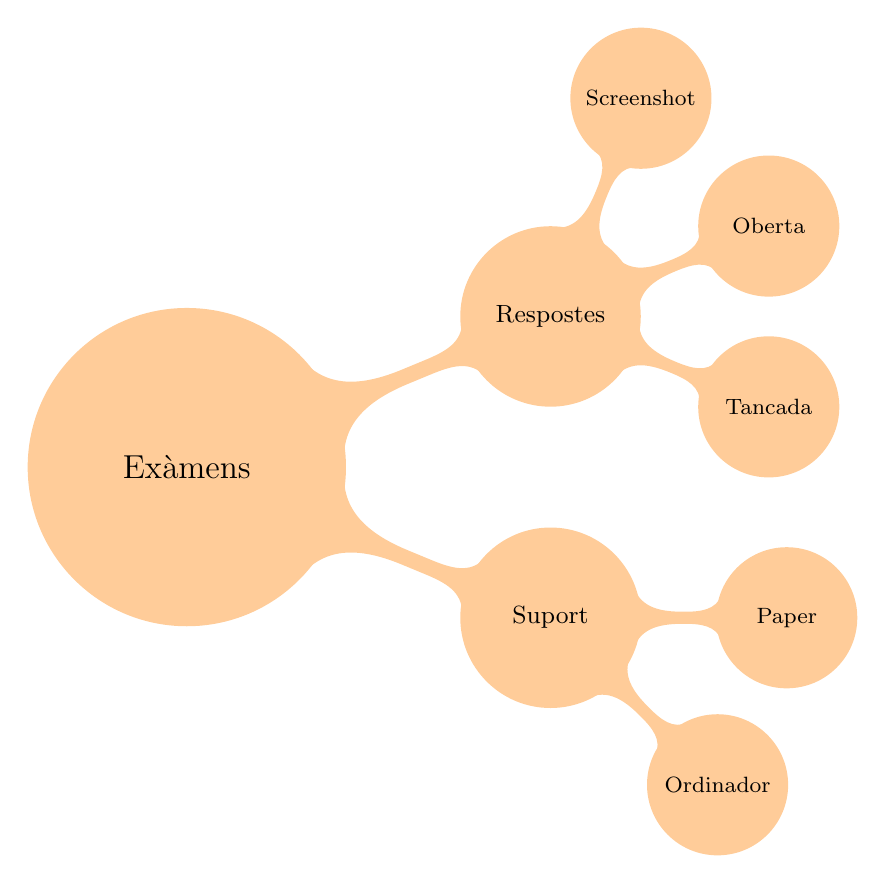
\begin{tikzpicture}[mindmap, grow cyclic, every node/.style=concept, concept color=orange!40, 
	level 1/.append style={level distance=5cm,sibling angle=45},
	level 2/.append style={level distance=3cm,sibling angle=45},]

\node{Exàmens}
	  child{ node {Suport}
	    child{ node {Ordinador}}
	    child{ node {Paper}}
	  }
	  child{ node {Respostes}
	    child{ node {Tancada}}
	    child{ node {Oberta}}
	    child{ node {Screenshot}}
	  }
;
\end{tikzpicture}
\caption{Classificació dels exàmens individuals segons el tipus de suport i el tipus de resposta.} \label{fig:M1}
\end{figure}

Per a aquells alunes que no aprovin l'avaluació contínua es preparà un exàmen de recuperació ordinària al mes de juny i un examen de recuperació extrordinària. Cada un d'aquests exàmes tracta tot allò que s'ha fet durant el mòdul i, per tant, són exigents a causa del seu abast. Els alumnes han de saber el mecanisme habitual per aprovar el mòdul és l'avaluació contínua i els examens de recuperació són un mecanisme excepcional.

\subsection{Avaluació de la tasca docent}

De manera trimestral es demanarà als alumnes que reflexionin sobre el mòdul i la tasca docent. Aquesta informació s'utilitzarà per a intentar reorientar i millorar el mòdul en els trimestres següents i en les pròximes edicions del curs. 

\begin{itemize}
	\item Què és el més interessant que hem vist?
	\item Què és allò que ha quedat menys clar o que genera més dubtes?
	\item Què en penses del mòdul i de la tasca del professor?
	\item Què es podria fer per millorar?
\end{itemize}



\section{Activitats.}

Les activitats inclouen material per l'autoavaluació, tasques avaluables pel professor i exàmens.
Aquestes activitats són diverses.
Qualcunes es plantegen com a treballs on els alumnes han de cercar informació.
Altres consisteixen en seguir una sèrie de passes i presentar un informe.
També n'hi ha on l'enunciat presenta un problema o repte que els alumnes han de resoldre.

La majoria de les tasques de classe són per parelles o grups, mentre que els exàmens són individuals.
A la secció \ref{sec:instruments} ja hem detallat com són els exàmens.

La secció \ref{sec:continguts} detalla les activitats de cada una de les unitats didàctiques mentre que la calendarització orientativa es troba a l'appèndix \ref{app:schedule}.

\section{Metodologia.}

Segons el Real Decret 1147/2011, de 29 de juliol, pel que s'estableix l'ordenació general de formació professional del sistema educatiu, la metodologia didàctica de les ensenyances de formació professional integrarà els aspectes científics, tecnològics i organitzatius que correponguin en cada cas, amb la finalitat que l'alumnat adquireixi una visió global dels processos productius de l'activitat professional corresponent.

Es prioritzaran aquelles metodologies en les que l'alumne sigui el protagonista. Especialment, la realització de tasques per parelles en les que els alumnes puguin ``aprendre fent'' (learn by doing) i aprendre també dels seus companys.

El professor farà breus presentacions seguint el format de classe magistral quan sigui imprescindible, habitualment per a la introducció i la contextualització d'un tema.
Sempre que sigui possible, els alumnes aprendran realitzant tasques, discuntint-les i presentant-les.
Així mateix, s'espera que durant aquestes tasques sorgeixin dubtes. 
A vegades serà possible per als alumnes resoldre-les de manera autònoma i consultant els companys, però quan això no sigui possible el professor ha d'intervenir fent totes les explicacions i aclariments que siguin necessaris per acompanyar als alumnes pel bon camí de l'aprenentatge.

Es fomentarà el treball en parelles ja que el treball en equip és una habilitat fonamental que s'ha de practicar.
A més, permentent que els alumnes treballin per parelles es poden presentar tasques d'un nivell de dificultat més alt i els alumnes avancen més ràpid ja que si un s'equivoca o no sap com continuar, probablement l'altre sí que ho farà bé.

Que el treball sigui per parelles no significa que no pugui treballar tota la classe com un únic equip.
Al contrari, s'animarà als alumnes que s'ajudin uns grups als altres i fins i tot que prenguin temporalment el rol de professor per explicar qualque cosa a tota la classe.
De totes maneres cada parella es responsabilitza de realitzar la seva tasca de manera completa i d'entregar un informe detallat documentant el procés.

No és acceptable que una parella es divideixi la pràctica en dues parts i cada membre treballi de manera independent sense conèixer allò que fa l'altre. 
Cada integrant de la parella ha de tenir un coneixement total de la seva pràctica i ser capaç de respondre les preguntes del professor i de la resta de companys de classe.

Les pràctiques que es plantegen normalment tenen dues parts.
La primera part és formada per una sèrie de requisits plantejats pel professor i que la pràctica ha de complir. 
Aquesta part serveix per aprovar i per obtenir el 50\% de la nota.
La segona part de la pràctica és oberta i els alumnes, seguint el seu bon criteri, han d'anar més enllà d'allò que els demana el professor.
Explorar possibilitats que no s'encabeixen, o tan sols es suggereixen, a l'enunciat de la pràctica.
Aquesta segona part de la pràctica és imprevisible per al professor i els alumnes la completaran en funció dels seus coneixements adquirits fora de la classe de l'assignatura, els seus interessos, etc.
La segona part de la pràctica permet als alumnes optar a un 50\% addicional de la nota i, per tant, treure bona nota.

S'ha de reconèixer que aquest plantejament sovint topa, al principi, amb les expectatives de l'alumnat.
A l'inici del curs és natural que els alumnes arribin amb una mentalitat de fer el mínim possible i treure la màxima nota.
``Com pot ser que no tengui la nota màxima si he fet els requisits mínims que em demana l'enunciat?'' es una pregunta habitual a principi de curs.
A la llarga, aquells alumnes amb més iniciativa agraeixen la llibertat de tenir una pràctica oberta i assumeixen el repte de fer propostes que els permetin millorar la seva pràctica per obtenir bones notes.
És natural consultar abans amb el professor. 
Els alumnes preguntaran al professor, per exemple ``Creus que és una bona idea ampliar la pràctica tractant aquest aspecte que no hem vist a classe?''.
L'objectiu final és que els alumnes siguin els protagonistes i els que tenen la iniciativa en el procés d'ensenyament-aprenentatge.

De la mateixa manera, el professor ha d'estar preparat per fer concessions, sempre que siguin raonables, per adaptar el curs a allò que desitgen els alumnes.
També hi ha certa flexibilitat pel que fa al ritme de l'assignatura. 
Si els alumnes estan molt engrescats en una pràctica, o tenen especial dificultat, s'ajustaran els terminis d'entrega en uns límits raonables.
La regla d'or és que si treballen durant tota la classe i no poden acabar la tasca encomanada, el professor pot concedir més temps per acabar-la.
Evidentment, els alumnes no poden demanar allargar els terminis d'entrega si no s'aprofiten bé el temps de classe.

S'intenta establir un clima de diàleg i consens per tal que la càrrega de feina de l'assignatura sigui proporcional al número d'hores assignades setmanalment.

\subsection{Presencial, semipresencial i a distància}

Una programació didàctica ha de ser prou àgil per adaptar-se als diferents escenaris de presencilalitat.
A causa d'una pandèmia o per altres motius, és possible que part o la totalitat dels alumnes no puguin assistir a part o la totalitat de les classes presencials.
Per aquest motiu s'ha dissenyat un curs que permet el seu seguiment en els escenaris semipresencial i d'ensenyament a distància.

\subsection{Recursos materials}

L'ordre EDU/392/2010 per la que s'estableix el currículum del cicle formatiu de Grau Superior corresponent al títol de Tècnic Superior en Administració de Sistemes Informàtics en Xarxa, en el seu annex IV, especifica els espais i equipaments mínims per al cicle.

A la pràctica, es necessita un ordinador amb connexió a internet i prou potent per poder utilitzar un navegador modern. També un compte de \emph{g-suite for education} per a cada alumne. S'utilitzarà google classroom com a plataforma d'e-learning i google cloudshell per a la realització de les pràctiques. És desitjable que els ordinadors puguin executar contenidors i màquines virtuals per tenir una alternativa a google cloudshell. Per a les proves en paper es necessitarà un bolígraf.

També es necessita un projector i una pissarra.

En cas de semipresencialitat o ensenyament a distància s'emprarà també una eina de comunicació addicional, com per exemple el discord.

\section{Distribució temporal.}

Segons l'annex II de l'Ordre EDU/392/2010, de 20 de gener, per la que s'estableix el currículum del cicle formatiu de Grau Superior corresponent al títol de Tècnic Superior en Administració de Sistemes Informàtics en Xarxa, al mòdul de gestió de Bases de Dades li correponen 170 hores de duració. A aquestes hores se li han de sumar les 90 reservades als mòduls impartits en anglès. El total és de 260 hores.

Segons el mateix annex, al mòdul li corresponen 5 hores anuals més unes altres 3 per ser en anglès. En total la suma és 8 hores setmanals.

En qualsevol cas, la distribució temporal que s'ofereix a continució és orientativa i s'ajustarà al calendari escolar. També s'anirà adaptant durant el desenvolupament del curs per ajustar-se al grup d'alumes i les altres circumstàncies de contexte.

La Taula \ref{tab:distribuciotemporal} mostra la proposta de distribució temporal orientativa.

\begin{table}
	\centering
\begin{tabular}{lr}
 Títol & Hores\\
 \hline
 Unit 1: Introduction to Databases. & 16\\
 Unit 2: Introduction to the Relational Model. & 20  \\
 Unit 3: Introduction to SQL 1. & 20\\
 Unit 4: Introduction to SQL 2. & 20 \\
 Unit 5: Intermediate SQL 1. & 20 \\
 Unit 6: Intermediate SQL 2. & 20 \\
 Unit 7: Advanced SQL 1. & 24 \\
 Unit 8: Advanced SQL 2. & 24\\
 Unit 9: Database Design. The E-R Model 1 & 24\\
 Unit 10: Database Design. E-R Model to Relation Model & 24 \\
 Unit 11: Database Design. Normalizarion & 24 \\
 Unit 12: Advanced Topics. & 24 \\
\end{tabular}
	\caption{Distribució temporal de la programació} \label{tab:distribuciotemporal}
\end{table}

La calendarització orientativa, allò que tenim planificat fer cada dia de classe, es presenta a l'appèndix \ref{app:schedule}.

\section{Continguts, activitats i recursos per a les unitats didàctiques.}
\label{sec:continguts}

A l'hora de dissenyar un curs introductori de base de dades, hi ha dues aproximacions possibles.
La primera, potser més habitual a la formació professional, és programar el disseny de base dades (entitat relació, relacional) abans que el llenguatge SQL.
La segona alternativa, igualment vàlida, és ensenyar SQL abans que la metodologia de disseny de les bases de dades.
En aquesta programació didàctica s'ha elegit la segona opció.

Un dels motius, és que aquest és l'ordre seguit en el llibre de referència elegit per a aquesta signatura, el de Silbershatz \cite{silbershatz2020}.
Un altre motiu de pes, és que els alumnes de dual necessiten saber SQL en el moment en que s'incorporen al seu lloc de feina.
Un informàtic també ha de saber dissenyar bases de dades, però quan un s'incorpora al món laboral és més probable que ho faci treballant amb queries que no dissenyant bases de dades, que és una tasca que habitualment fan informàtics amb més experiència.
A més, la part de disseny de base de dades i normalització, que pot ser més abstracta, s'entén millor una vegada els alumnes ja tenen uns mesos d'experiència en bases de dades.
Durant la seva fomació de SQL, els alumnes es familiaritzen amb bases de de dades d'exemple, com una base de dades d'una escola, d'una empresa, etc.
Aquest coneixement previ els permet comprendre millor les unitats de treball relacionades amb el disseny de base de dades.

A continuació es descriuen cada una de les dotze unitats de treball d'aquesta programació.

  \subsection{Unit 1: Introduction to Databases}
  
  \subsubsection{Contents}

  \begin{itemize}
	  \item Database-System Applications
	  \item Purpose of Database Systems
	  \item View of Data
	  \item Database Languages
	  \item Relational Databases
	  \item Database Design
	  \item Data Storage and Querying
	  \item Transaction Management
	  \item Database Architecture
	  \item Data Mining and Information Retrieval
	  \item Specialty Databases
	  \item Database Users and Administrators
	  \item History of Database Systems
  \end{itemize}
  
  \subsubsection{Material}

  \begin{itemize}
          \item Slides 1-1 Introduction to Databases.
	  \item Assignment 1-1 Introduction to Databases.
		  (\faGraduationCap Evaluation criteria) 1a, 1b, 1c, 1d, 1e, 1f.
	  \item Test 1 Introduction to Databases.
  \end{itemize}

  \subsection{Unit 2: Introduction to the Relational Model}

  \subsubsection{Contents}

  \begin{itemize}
	  \item Structure of Relational Databases
	  \item Database Schema
	  \item Keys
	  \item Schema Diagrams
	  \item Relational Query Languages
	  \item Relational Operations
  \end{itemize}

  \subsubsection{Material}

  \begin{itemize}
          \item Slides 2-1 Introduction to the Relational Model.
	  \item Assignment 2-1 Installing a Relational Database.
	  \item Assignment 2-2 Keys. (\faGraduationCap Evaluation criteria) 2f
	  \item Assignment 2-3 Relational Diagram. (\faGraduationCap Evaluation criteria) 2b
	  \item Assignment 2-4 Relational Algebra.
	  \item Test 2 Introduction to the Relational Model.
  \end{itemize}

  \subsection{Unit 3: Introduction to SQL 1}

  \subsubsection{Contents}
  \begin{itemize}
	  \item Overview of the SQL Query Laguage
	  \item SQL Data Definition
	  \item Basic Structure of SQL Queries
	  \item Additional Basic Operations
	  \item Set Operations
  \end{itemize}

  \subsubsection{Material}

  \begin{itemize}
	  \item Slides 3-1 Introduction to SQL 1.
	  \item Assignment 3-1 Create a Database. (\faGraduationCap Evaluation criteria) 3a, 3b, 3c, 3d.
	  \item Assignment 3-2 A Dockerized Database.
	  \item Assignment 3-3 School Database Script. (\faGraduationCap Evaluation criteria) 4a, 4b, 5a, 5b, 5d.
	  \item Test 3 Introduction to SQL 1.
  \end{itemize}

  \subsection{Unit 4: Introduction to SQL 2}

  \subsubsection{Contents}
  \begin{itemize}
	  \item Null Values
	  \item Aggregate Functions (\faGraduationCap Evaluation criteria) 4c
	  \item Nested Subqueries
	  \item Modifications of the Database
  \end{itemize}
  
  \subsubsection{Material}

  \begin{itemize}
	  \item Slides 4-1 Introduction to SQL 2.
	  \item Material 4-1 Queries MariaDB. (\faGraduationCap Evaluation criteria) 4f.
	  \item Material 4-2 Queries MariaDB. (\faGraduationCap Evaluation criteria) 4g, 5c.
	  \item Material 4-3 Northwind.
	  \item Test 4 Introduction to SQL 2.
  \end{itemize}

  \subsection{Unit 5: Intermediate SQL 1}

  \subsubsection{Contents}

  \begin{itemize}
	  \item Join Expressions
	  \item Views
	  \item Transactions
  \end{itemize}

  \subsubsection{Material}

  \begin{itemize}
	  \item Slides 5-1 Intermediate SQL 1.
	  \item Assignment 5-1 Dockerized phpMyAdmin.
	  \item Material 5-1 Join. (\faGraduationCap Evaluation criteria) 4d, 4e.
	  \item Material 5-2 View.
	  \item Material 5-3 Transactions. (\faGraduationCap Evaluation criteria) 5f 5g.
	  \item Material 5-4 Transactions.
	  \item Assignment 5-1 Two-phase locking and snapshop isolation. (\faGraduationCap Evaluation criteria) 5g.
	  \item Test 5 Intermediate SQL 1.
  \end{itemize}

  \subsection{Unit 6: Intermediate SQL 2}
  
  \subsubsection{Contents}
  \begin{itemize}
	  \item Integrity Constraints
	  \item Data Types
	  \item Authorization
  \end{itemize}

  \subsubsection{Material}
  \begin{itemize}
	  \item Slides 6-2 Intermediate SQL 1.
	  \item Material 6-1 Referential integrity and data types.
	  \item Assignment 6-1 Mini League.
	  \item Material 6-2 Index Importance.
	  \item Material 6-3 Authorization.
	  \item Material 6-4 Roles.
	  \item Material 6-5 Dates.
	  \item Material 6-6 Database for Test 6.
	  \item Test 6 Intermediate SQL.

  \end{itemize}
  

  \subsection{Unit 7: Advanced SQL 1}
  
  \subsubsection{Contents}
  \begin{itemize}
	  \item SQL statements in a java application
  \end{itemize}

  \subsubsection{Material}
  \begin{itemize}
	  \item Material 7-1 SQL statements in a java application.
	  \item Assignment 7-1 JDBC Project.
	  \item Assignment 7-2 JDBC Project Video Explanationand Demonstration.
  \end{itemize}

  \subsection{Unit 8: Advanced SQL 2}

  \subsubsection{Contents}
  \begin{itemize}
	  \item Cursors
	  \item Procedures
	  \item Triggers
  \end{itemize}

  \subsubsection{Material}
  \begin{itemize}
	  \item Material 8-1 PostgreSQL.
	  \item Material 8-2 PostgreSQL Stored Procedures Getting Started. (\faGraduationCap Evaluation criteria) 5e.
	  \item Material 8-3 PostgreSQL Stored Procedures User Defined Functions.
	  \item Material 8-4 PostgreSQL Stored Procedures Control Structures.
	  \item Assignment 8-1 Create a Function.
	  \item Assignment 8-2 Function Defense.
	  \item Assignment 8-3 Create a Cursor, a Stored Procedure and a Trigger.
	  \item Assignment 8-4 Defend your Cursor, Procedure and Trigger.
  \end{itemize}

  \subsection{Unit 9: Database Design. The E-R Model 1}

  \subsubsection{Contents}
  \begin{itemize}
	  \item Entity-Relationship Model
	  \item Entity-Relationship Diagram
	  \item Cardinalities
	  \item Weak Entities
	  \item Extended E-R, Generalization and Specialization
  \end{itemize}

  \subsubsection{Material}
  \begin{itemize}
	  \item Material 9-1 Slides.
	  \item Material 9-2 E-R Diagram Tool.
	  \item Assignment 9-1 Create an ERD. (\faGraduationCap Evaluation criteria) 2a, 2b.
	  \item Assignment 9-2 Defend your ERD.
  \end{itemize}


  \subsection{Unit 10: Database Design. E-R Model to Relational Model.}

  \subsubsection{Contents}
  \begin{itemize}
	\item Reduction to Relational Schemas
  \end{itemize}

  \subsubsection{Material}
  \begin{itemize}
	  \item Assignment 10-1 ERM to Relational Model. (\faGraduationCap Evaluation criteria) 2c, 2d, 2e, 2f, 2g, 2i, 3e, 3f, 3g, 3h, 3i.
	  \item Assignment 10-2 Defend your Relational Model.
  \end{itemize}

  \subsection{Unit 11: Database Design. Normalization.}

  \subsubsection{Contents}
  \begin{itemize}
	\item Functional Dependency
	\item Fully Functional Dependency
	\item First Normal Form
	\item Second Normal Form
	\item Third Normal Form
	\item Boyce-Codd Normal Form
  \end{itemize}

  \subsubsection{Material}
  \begin{itemize}
	  \item Material 11-1 Slides (Simplified).
	  \item Material 11-2 Slides.
	  \item Material 11-3 Exercises.
	  \item Material 11-4 Example of Solution.
	  \item Assignment 11-1 Normalization. (\faGraduationCap Evaluation criteria) 2h.
	  \item Assignment 11-2 Defend your Normalization.
  \end{itemize}


  \subsection{Unit 12: Advanced Topics.}

  \begin{itemize}
	\item Backup and restoration.
	\item Import and export data.
	\item Error messages and log files.
	\item Moving data across DataBase Management Systems.
	\item NoSQL databases.
  \end{itemize}

  \subsubsection{Material}
  \begin{itemize}
	  \item Assignment 12-1 Advanced Topics. (\faGraduationCap Evaluation criteria 6a, 6b, 6c, 6d, 6e, 6f, 6g, 6h).
	  \item Material 12-1 NoSQL.
  \end{itemize}


\section{Mesures per a l'atenció a la diversitat}

Al tractar-se d'un ensenyament post-obligatori no es contempla la possibilitat de prendre mesures d'adaptació curricular significatives. Es prendran mesures que no impliquin una modificació substancial del currículum amb l'assessorament del departament d'orientació.

Algunes mesures habituals poden ser cedir a les persones amb necessitats especials aquells llocs de la classe que els siguin més favorables o adaptar els temps de les proves a les seves necessitats.

Excepte en els exàmens, s'afavorirà el treball en equip de tal manera que les fortaleses d'uns puguin compensar les mancances d'uns altres. S'afavorirà un clima de col·laboració on les diferències siguin una oportunitat i no un obstacle.

Les persones amb necessitats especials sovint necessiten una atenció personalitzada, però a la pràctica no disposem de personal de suport a l'aula per atendre-les.
La solució és que siguin els mateixos companys de classe els que ajudin a qui ho necessita.
Quan assignam una tasca, qualcuns alumnes són capaços d'acabar molt abans que els altres per diferents motius.
Demanarem a aquest alumnes que donin un cop de mà als que vagin més lents.

Aquesta estratègia té múltiples avantatges. 
Per una part, mitiga el problema que suposa que uns acabin molt abans que els altres.
A més, els alumnes amb necessitats especials poden rebre un tracte personalitzat i dedicat per part d'un company.
Aquest company pot explicar les coses de manera més propera i diferent de com ho ha fet el professor per ajudar a entendre conceptes.
Els avantatges no són només per a la persona ajudada, també per a la que ajuda.
L'alumne que ajuda als companys consolida els seus propis coneixements i amb això obtindrà també millors notes.

A més, a l'aula trobam persones amb diferents fortaleses i debilitats.
Els que un dia són ajudats en una altra ocasió potser seran ajudants i així es canviaran el rols.
Finalment, es comença a treballar amb un model que és molt habitual en el món de les tecnologies de la informació anomenat ``meritocràcia''.
En una meritocràcia, aquells que més aporten al projecte es guanyen el respecte dels companys i la seva veu és escoltada amb especial atenció a l'hora de prendre decisions.

\section{Conclusió}

Aquesta programació didàctica descriu la planificació per al mòdul de gestió de bases de dades en anglès.
Està contextualitzada per a un cicle en concret (ASIX) d'un centre en concret (CIFP Francesc de Borja Moll).

El marc legal ens marca uns objectius, unes competències, i uns resultats d'aprenentatge lligats a uns criteris d'avaluació.

Quant a metodologies, hem prioritzat aquelles reforcen el protagonisme dels alumnes.
Trantant-se de formació professional, és adequat assignar tasques als alumnes que s'aproximen a les que es podrà trobar en el centre de treball.
Per descomptat, en un entorn favorable per a l'aprenentatge amb el suport dels companys de classe i del professor.

La distribució temporal és orientativa i flexible.
Es pot anar ajustar depenent dels alumnats, els coneixements previs que disposen o el seu interés per les diferents temàtiques.
S'ha decidit tractar primer les unitats de treball relacionades amb SQL i posteriorment aquelles que estan relacionades amb el disseny de les bases de dades.
El motiu és que les tasques que es trobaran al incorporar-se al centre de treball probablement estaran relacionades amb queries sobre una base de dades existent més que no en el disseny de noves bases de dades, que habitualment són tasques reservades als analistes o personal amb més experiència.o

Els continguts i les orientacions pedagògiques ens venen marcats per la normativa.
Tot i això, sempre hi ha un poc de marge per emfatitzar aquells aspectes que creguem que poden ser de més interés en funció de les tecnologies més utilitzades per les organitzacions on s'incorporaran els alumnes a treballar.

Quant a l'avaluació s'ha optat per tenir en compte tant les tasques com els exàmens.
A més, les tasques i els exàmens seran de naturalesa diferent.
El motiu és fer una avaluació amb un gran abast.
En altres paraules, si un alumne té dificultats amb un aspecte concret de l'avaluació (per exemple, l'expressió oral), aquestes dificultats es veuran compensades per les seves fortaleses en els altres mecanismes d'avaluació.
A més, es mantendrà un clima de diàleg i flexibilitat perquè els alumnes puguin avaluar la tasca docent i fer suggeriments per millorar-la.

Així mateix, es farà una atenció personalitzada per a l'alumnat.
També s'animarà al suport mutu dins el grup perquè els mateixos alumnes participin en l'atenció a la diversitat en la mesura possible.

Es mantendrà un diàleg obert amb l'alumnat i altres professors per reforçar la interconnexió entre els diferents mòduls.
Tot i que per motius pràctics els continguts del cicle s'organitzen en mòduls independents, en realitat tots aquests continguts presenten lligams per es poden aprofitar per a oferir una millor experiència d'ensenyament-aprenentatge.

A més dels continguts propis del cicle, es treballaran uns elements transversals que són també de gran importància per a la formació de l'alumnat. 
S'han elegit el resepecte pels valors cívics, els hàbits de vida saludable, el foment de la lectura de la documentació tècnica i la generació de documentació escrita i la seva presentació de manera oral.

Els continguts del cicle s'han organitzat en 12 unitats de treball.
Cada una d'elles es composa de materials, tasques (assignments) i proves (tests) d'avaluació.

\section{Bibliografia}

És de gran utilitat tenir un llibre de referència per al curs.
Per una banda, ajuda al professor a preparar millor el curs.
Per una altra, és un recurs addicional per a l'alumne per a poder seguir el curs de manera més autònoma.
Un llibre d'interès és \cite{montalban2014}.
L'avantatge d'aquest llibre és que s'ajusta molt al currículum oficial.

El llibre que s'ha adoptat com a referència per a aquest curs és \cite{silbershatz2020}.
És un dels llibres de bases dades més reconeguts i s'utilitza a multitud de centres d'arreu del món.
Els diferents conceptes es van introduint amb gran rigor i claretat.
El desavantatge que té aquest llibre és que està orientat a un curs universitari i, per tant, no s'ajusta tan bé al currículum de la formació professional.
Per tant, en el nostre curs no veurem tot allò que és el llibre.
A més, completarem el llibre amb altres materials més pràctics com per exemple la documentació de postgresql.

\begin{thebibliography}{9}

\bibitem{coll2017} 
J. Coll Amengual
\textit{La programació didàctica a ESO i Batxillerat}. 


\bibitem{montalban2014} 
I. López Montalbán, M. de Castro Vázquez
\textit{Gestión de Bases de Datos}. 
Editorial Garceta

\bibitem{silbershatz2020} 
A. Silbershatz, H. F. Korth i S. Sudarshan 
\textit{Database System Concepts}. 
McGraw Hill Education

\end{thebibliography}


\appendix

\section{Tentative Schedule}
\label{app:schedule}

\paragraph*{Tentative Schedule:}
\begin{center}
\begin{calendar}{9/23/2019}{40} % Semester starts on 1/11/2010 and last for 16
                    % weeks, including finals week
\setlength{\calboxdepth}{.3in}
\MTRFClass
% schedule
\caltexton{1}{1.1 Welcome. Presentation.}
\caltextnext{1.2 Slides}
\caltextnext{1.3 Assignment 1}
\caltextnext{1.4 Slides}
\caltextnext{1.5 Assignment 1}
\caltextnext{1.6 Review}
\caltextnext{1.7 Test}
\caltextnext{1.8 Test correction}
\caltextnext{2.1}
\caltextnext{2.2}
\caltextnext{2.3}
\caltextnext{2.4}
\caltextnext{2.5}
\caltextnext{2.6}
\caltextnext{2.7}
\caltextnext{2.8 Review}
\caltextnext{2.9 Test}
\caltextnext{2.10 Test correction}
\caltextnext{3.1}
\caltextnext{3.2}
\caltextnext{3.3}
\caltextnext{3.4}
\caltextnext{3.5}
\caltextnext{3.6}
\caltextnext{3.7}
\caltextnext{3.8 Review}
\caltextnext{3.9 Test}
\caltextnext{3.10 Test correction}
\caltextnext{4.1}
\caltextnext{4.2}
\caltextnext{4.3}
\caltextnext{4.4}
\caltextnext{4.5}
\caltextnext{4.6}
\caltextnext{4.7}
\caltextnext{4.8 Review}
\caltextnext{4.9 Test}
\caltextnext{4.10 Test correction}
\caltextnext{5.1}
\caltextnext{5.2}
\caltextnext{5.3}
\caltextnext{5.4}
\caltextnext{5.5}
\caltextnext{5.6}
\caltextnext{5.7}
\caltextnext{5.8 Review}
\caltextnext{5.9 Test}
\caltextnext{5.10 Test correction}
\caltextnext{6.1}
\caltextnext{6.2}
\caltextnext{6.3}
\caltextnext{6.4}
\caltextnext{6.5}
\caltextnext{6.6}
\caltextnext{6.7}
\caltextnext{6.8 Review}
\caltextnext{6.9 Test}
\caltextnext{6.10 Test correction}
\caltextnext{7.1}
\caltextnext{7.2}
\caltextnext{7.3}
\caltextnext{7.4}
\caltextnext{7.5}
\caltextnext{7.6}
\caltextnext{7.7}
\caltextnext{7.8}
\caltextnext{7.9}
\caltextnext{7.10}
\caltextnext{7.11 Presentations}
\caltextnext{7.12 Presentations}
\caltextnext{8.1}
\caltextnext{8.2}
\caltextnext{8.3}
\caltextnext{8.4}
\caltextnext{8.5}
\caltextnext{8.6}
\caltextnext{8.7}
\caltextnext{8.8}
\caltextnext{8.9}
\caltextnext{8.10}
\caltextnext{8.11 Presentations}
\caltextnext{8.12 Presentations}
\caltextnext{9.1}
\caltextnext{9.2}
\caltextnext{9.3}
\caltextnext{9.4}
\caltextnext{9.5}
\caltextnext{9.6}
\caltextnext{9.7}
\caltextnext{9.8}
\caltextnext{9.9}
\caltextnext{9.10}
\caltextnext{9.11 Presentations}
\caltextnext{9.12 Presentations}
\caltextnext{10.1}
\caltextnext{10.2}
\caltextnext{10.3}
\caltextnext{10.4}
\caltextnext{10.5}
\caltextnext{10.6}
\caltextnext{10.7}
\caltextnext{10.8}
\caltextnext{10.9}
\caltextnext{10.10}
\caltextnext{10.11 Presentations}
\caltextnext{10.12 Presentations}
\caltextnext{11.1}
\caltextnext{11.2}
\caltextnext{11.3}
\caltextnext{11.4}
\caltextnext{11.5}
\caltextnext{11.6}
\caltextnext{11.7}
\caltextnext{11.8}
\caltextnext{11.9}
\caltextnext{11.10}
\caltextnext{11.11 Presentations}
\caltextnext{11.12 Presentations}
\caltextnext{12.1}
\caltextnext{12.2}
\caltextnext{12.3}
\caltextnext{12.4}
\caltextnext{12.5}
\caltextnext{12.6}
\caltextnext{12.7}
\caltextnext{12.8}
\caltextnext{12.9}
\caltextnext{12.10}
\caltextnext{12.11 Presentations}
\caltextnext{12.12 Presentations}
% ... and so on

% Holidays
\Holiday{10/12/2019}{Pilar}
\Holiday{11/1/2019}{Tots Sants}
\Holiday{12/6/2019}{Constitució}
\Holiday{12/8/2019}{Immaculada}
% ... and so on

\options{12/23/2019}{\noclassday} % finals week
\options{12/24/2019}{\noclassday} % finals week
\options{12/25/2019}{\noclassday} % finals week
\options{12/26/2019}{\noclassday} % finals week
\options{12/27/2019}{\noclassday} % finals week
\caltext{4/27/2010}{\textbf{Final Exam}}
\end{calendar}
\end{center}

\end{document}
